\chapter[SCP-005 万能钥匙]{
	SCP-005 - Skeleton Key\\
	SCP-005 - 万能钥匙
}

\label{chap:SCP-005}

\begin{figure}[H]
	\centering
	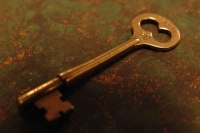
\includegraphics[width=0.5\linewidth]{images/SCP.005.jpg}
	\caption*{SCP-005的一张特写}
\end{figure}

\bb{项目编号:}SCP-005

\bb{项目等级:}Safe

\bb{特殊收容措施:}从直觉角度说,SCP-005没有显露出任何危险性。即便如此,它独特的功能也要求采取特殊措施限制接触及操作对象的权限。从管控区转移对象至少需要一名4级人员的许可。

\bb{描述:}从外观上看,SCP-005就是一把装饰华丽的钥匙,表现出20世纪20年代大规模生产的钥匙的典型特征。SCP-005被发现时,一名平民正用它潜入一栋守卫森严的设施。它似乎拥有可以轻而易举地打开任何形式的锁(见附录A)的能力,不论那锁是机械式的还是数字式的。该能力的来源目前依旧无法断定。

\bb{追加记录:}在至少一名4级人员的监督之下,SCP-005可用做丢失的安全通行证的替代品,但禁止用于自动贩卖机的修理、开启寄物柜或充当私人宅邸的备用钥匙。把对象移出围墙将面临就地处决。

\bb{附录A:}虽然SCP-005在解除任何形式的闩锁装置方面显得卓有成效,但进一步的实验却表明,掩饰锁的功用与特征的努力能在某种程度上令SCP-005变得毫无用武之地。在大约50\%的案例中,志愿者无法认出闩锁装置,SCP-005也就无法成功破解。基于这些试验结果,SCP-005暂时归入“有感知力”的类别,还要开展进一步的试验以测试其认识能力。可我们只了解到上述装置可以蒙混过关,却并不清楚究竟是哪些特征能够阻止其认出特定的锁。
